\subsection{Caso d'uso UC3: Ricerca di un progetto}
\begin{figure}[h] 
	\centering 
	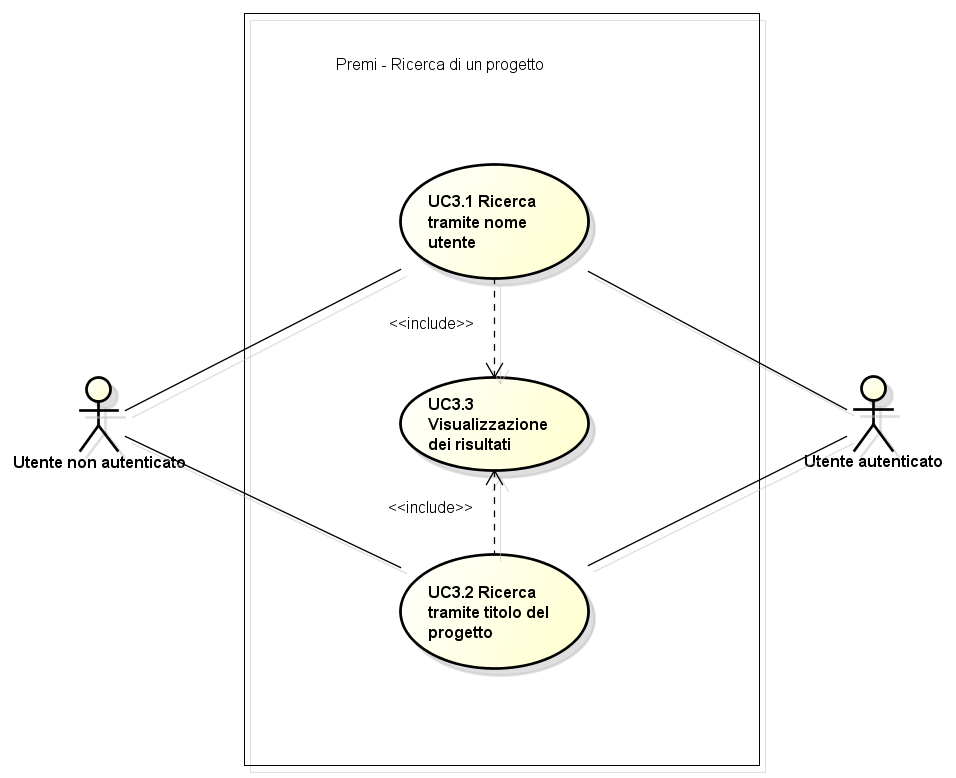
\includegraphics[scale=0.45] {img/UC3.png} 
	\caption{UC3 - Ricerca di un progetto} 
\end{figure}

\begin{itemize}
	\item \textbf{Attori:} Utente non autenticato, utente autenticato;
	\item \textbf{Scopo e descrizione:} L'utente può cercare un progetto utilizzando come chiave di ricerca il nome utente o il titolo del progetto;
	\item \textbf{Precondizione:} L'utente sta visualizzando la schermata di ricerca;
	\item \textbf{Flusso principale degli eventi:}
	\begin{enumerate}
		\item L'utente inserisce come chiave di ricerca il nome utente del creatore del progetto [UC3.1];
		\item L'utente inserisce come chiave di ricerca il titolo del progetto [UC3.2];
		\item Il sistema mostra all'utente i risultati della ricerca [UC3.3].
	\end{enumerate}
	\item \textbf{Postcondizione:} Il sistema mostra all'utente il risultato della ricerca.
\end{itemize}

\subsection{Caso d'uso UC3.1: Ricerca tramite nome utente}
\begin{itemize}
	\item \textbf{Attori:} Utente non autenticato, utente autenticato;
	\item \textbf{Scopo e descrizione:} L'utente inserisce nella casella di ricerca il nome utente di un creatore di un progetto;
	\item \textbf{Precondizione:} Il sistema mostra la schermata di ricerca;
	\item \textbf{Postcondizione:} L'utente ha inserito un nome utente nella casella di ricerca ed ha avviato la ricerca.
\end{itemize}

\subsection{Caso d'uso UC3.2: Ricerca tramite titolo del progetto}
\begin{itemize}
	\item \textbf{Attori:} Utente non autenticato, utente autenticato;
	\item \textbf{Scopo e descrizione:} L'utente inserisce nella casella di ricerca il titolo di un progetto;
	\item \textbf{Precondizione:} Il sistema mostra la schermata di ricerca;
	\item \textbf{Postcondizione:} L'utente ha inserito un titolo nella casella di ricerca ed ha avviato la ricerca.
\end{itemize}

\subsection{Caso d'uso UC3.3: Visualizzazione dei risultati}
\begin{itemize}
	\item \textbf{Attori:} Sistema;
	\item \textbf{Scopo e descrizione:} Dopo aver avviato la ricerca il sistema mostra all'utente la schermata dei risultati della ricerca effettuata;
	\item \textbf{Precondizione:} L'utente ha avviato la ricerca;
	\item \textbf{Postcondizione:} Il sistema mostra all'utente i risultati della ricerca.
\end{itemize}

